\iffalse
\documentclass[12pt]{article}
\usepackage{graphicx}
\usepackage{amsmath}
\usepackage{mathtools}
\usepackage{gensymb}
\usepackage[utf8]{inputenc}
\usepackage{float}
\newcommand{\mydet}[1]{\ensuremath{\begin{vmatrix}#1\end{vmatrix}}}
\providecommand{\brak}[1]{\ensuremath{\left(#1\right)}}
\providecommand{\norm}[1]{\left\lVert#1\right\rVert}
\newcommand{\solution}{\noindent \textbf{Solution: }}
\newcommand{\myvec}[1]{\ensuremath{\begin{pmatrix}#1\end{pmatrix}}}
\let\vec\mathbf

\begin{document}
\begin{center}
\textbf\large{CLASS-11 \\ CHAPTER-10 \\ STRAIGHT LINES}
\end{center}
\section*{Excercise 10.4}

\\
\fi
The parameters of the given line are
		\begin{align}
	\vec{n}=\myvec{\sqrt{3}\\1},
			c=-2
		\end{align}
		From the above, 
		\begin{align}
			\tan\theta&=-\sqrt{3}\\
		\implies \theta&=-60\degree
		\end{align}
		and 
		\begin{align}
			p=\frac{|c|}{\norm{\vec{n}}}=\frac{2}{2}=1
		\end{align}
\begin{figure}[H]
	\begin{center} 
	    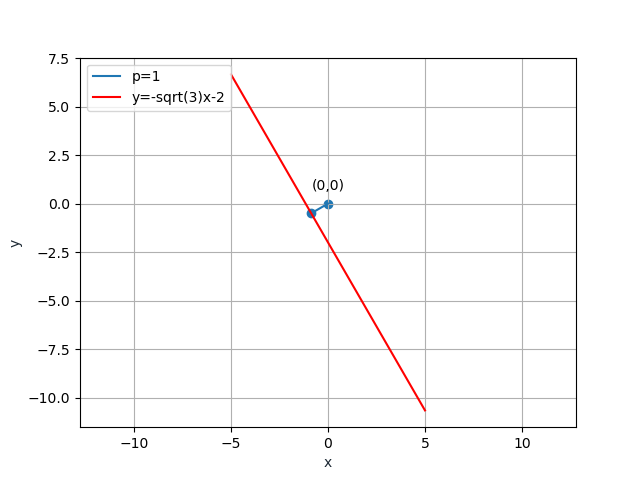
\includegraphics[width=\columnwidth]{chapters/11/10/4/2/figs/line.png}
	\end{center}
\caption{}
\label{fig:chapters/11/10/4/2/Fig1}
\end{figure}

